\chapter{Additional Tests}
\section{Effect of BHA Size}
A sensitivity test was conducted to assess the impact of the BHA size on drill string vibration. For this test, exaggerated sizes of BHA components were employed. All cases were based on Test Case 4 scenario. However, Test Case 4b\_A1, Test Case 4b\_A2, and Test Case 4b\_A3 were run with doubled outer diameter of BHA, tripled length of BHA, and both, respectively. \tablename~\ref{table_sensitivity_size_4b_input} summarizes the BHA properties for the sensitivity test.
\begin{table}
    \centering
    \begin{tabular}{|c|c|c|c|c|c|}
       \hline
       \textbf{Parameter} & \textbf{Test Case 4b} & \textbf{Test Case 4b\_A1} & \textbf{Test Case 4b\_A2} & \textbf{Test Case 4b\_A3}\\
       \hline
       $OD_{HWDP}$ & 0.1143 $m$ & 0.2286 $m$ & 0.1143 $m$ & 0.2286 $m$ \\
       \hline
       $ID_{HWDP}$ & 0.0635 $m$ & 0.0635 $m$ & 0.0635 $m$ & 0.0635 $m$ \\
       \hline
       $OD_{DC}$ & 0.1524 $m$ & 0.3048 $m$ & 0.1524 $m$ & 0.3048 $m$ \\
       \hline
       $ID_{DC}$ & 0.0508 $m$ & 0.0508 $m$ & 0.0508 $m$ & 0.0508 $m$ \\
       \hline
       $L_{HWDP}$ & 18.3 $m$ & 18.3 $m$ & 54.6 $m$ & 54.6 $m$ \\
       \hline
       $L_{DC}$ & 83.2 $m$ & 83.2 $m$ & 249.6 $m$ & 249.6 $m$ \\
       \hline
      \end{tabular}
    \caption[Input parameters for BHA size effect test for Test Case 4b]{Input parameters for BHA size effect test for Test Case 4b.}
    \label{table_sensitivity_size_4b_input}
\end{table}

The results presented in \figurename~\ref{figure_AS_BHA_size_effect_vel} and \ref{figure_AS_BHA_size_effect_td} demonstrate the influence of BHA size on angular velocity and torque, respectively. Increasing the diameter of the BHA significantly increased the maximum torque required to rotate the bit due to the increased inertia. On the other hand, the BHA length had an opposite effect, reducing the torque and increasing the vibration frequency. Combining both effects, enlarging both diameter and length of BHA, led to an increase in the torque required to rotate the bit and decreased the frequency of the vibration compared to simply increasing the diameter. In addition, when the BHA length was increased, comparing Test Case 4b and Test Case 4b\_A2, the sudden increase in bit angular velocity occurred after the stick phase, while it originally occurred right before the stick phase. Moreover, the spikes of the bit velocity below 0 $RPM$ occurred when the BHA length was increased.
\begin{figure}
  \centering
  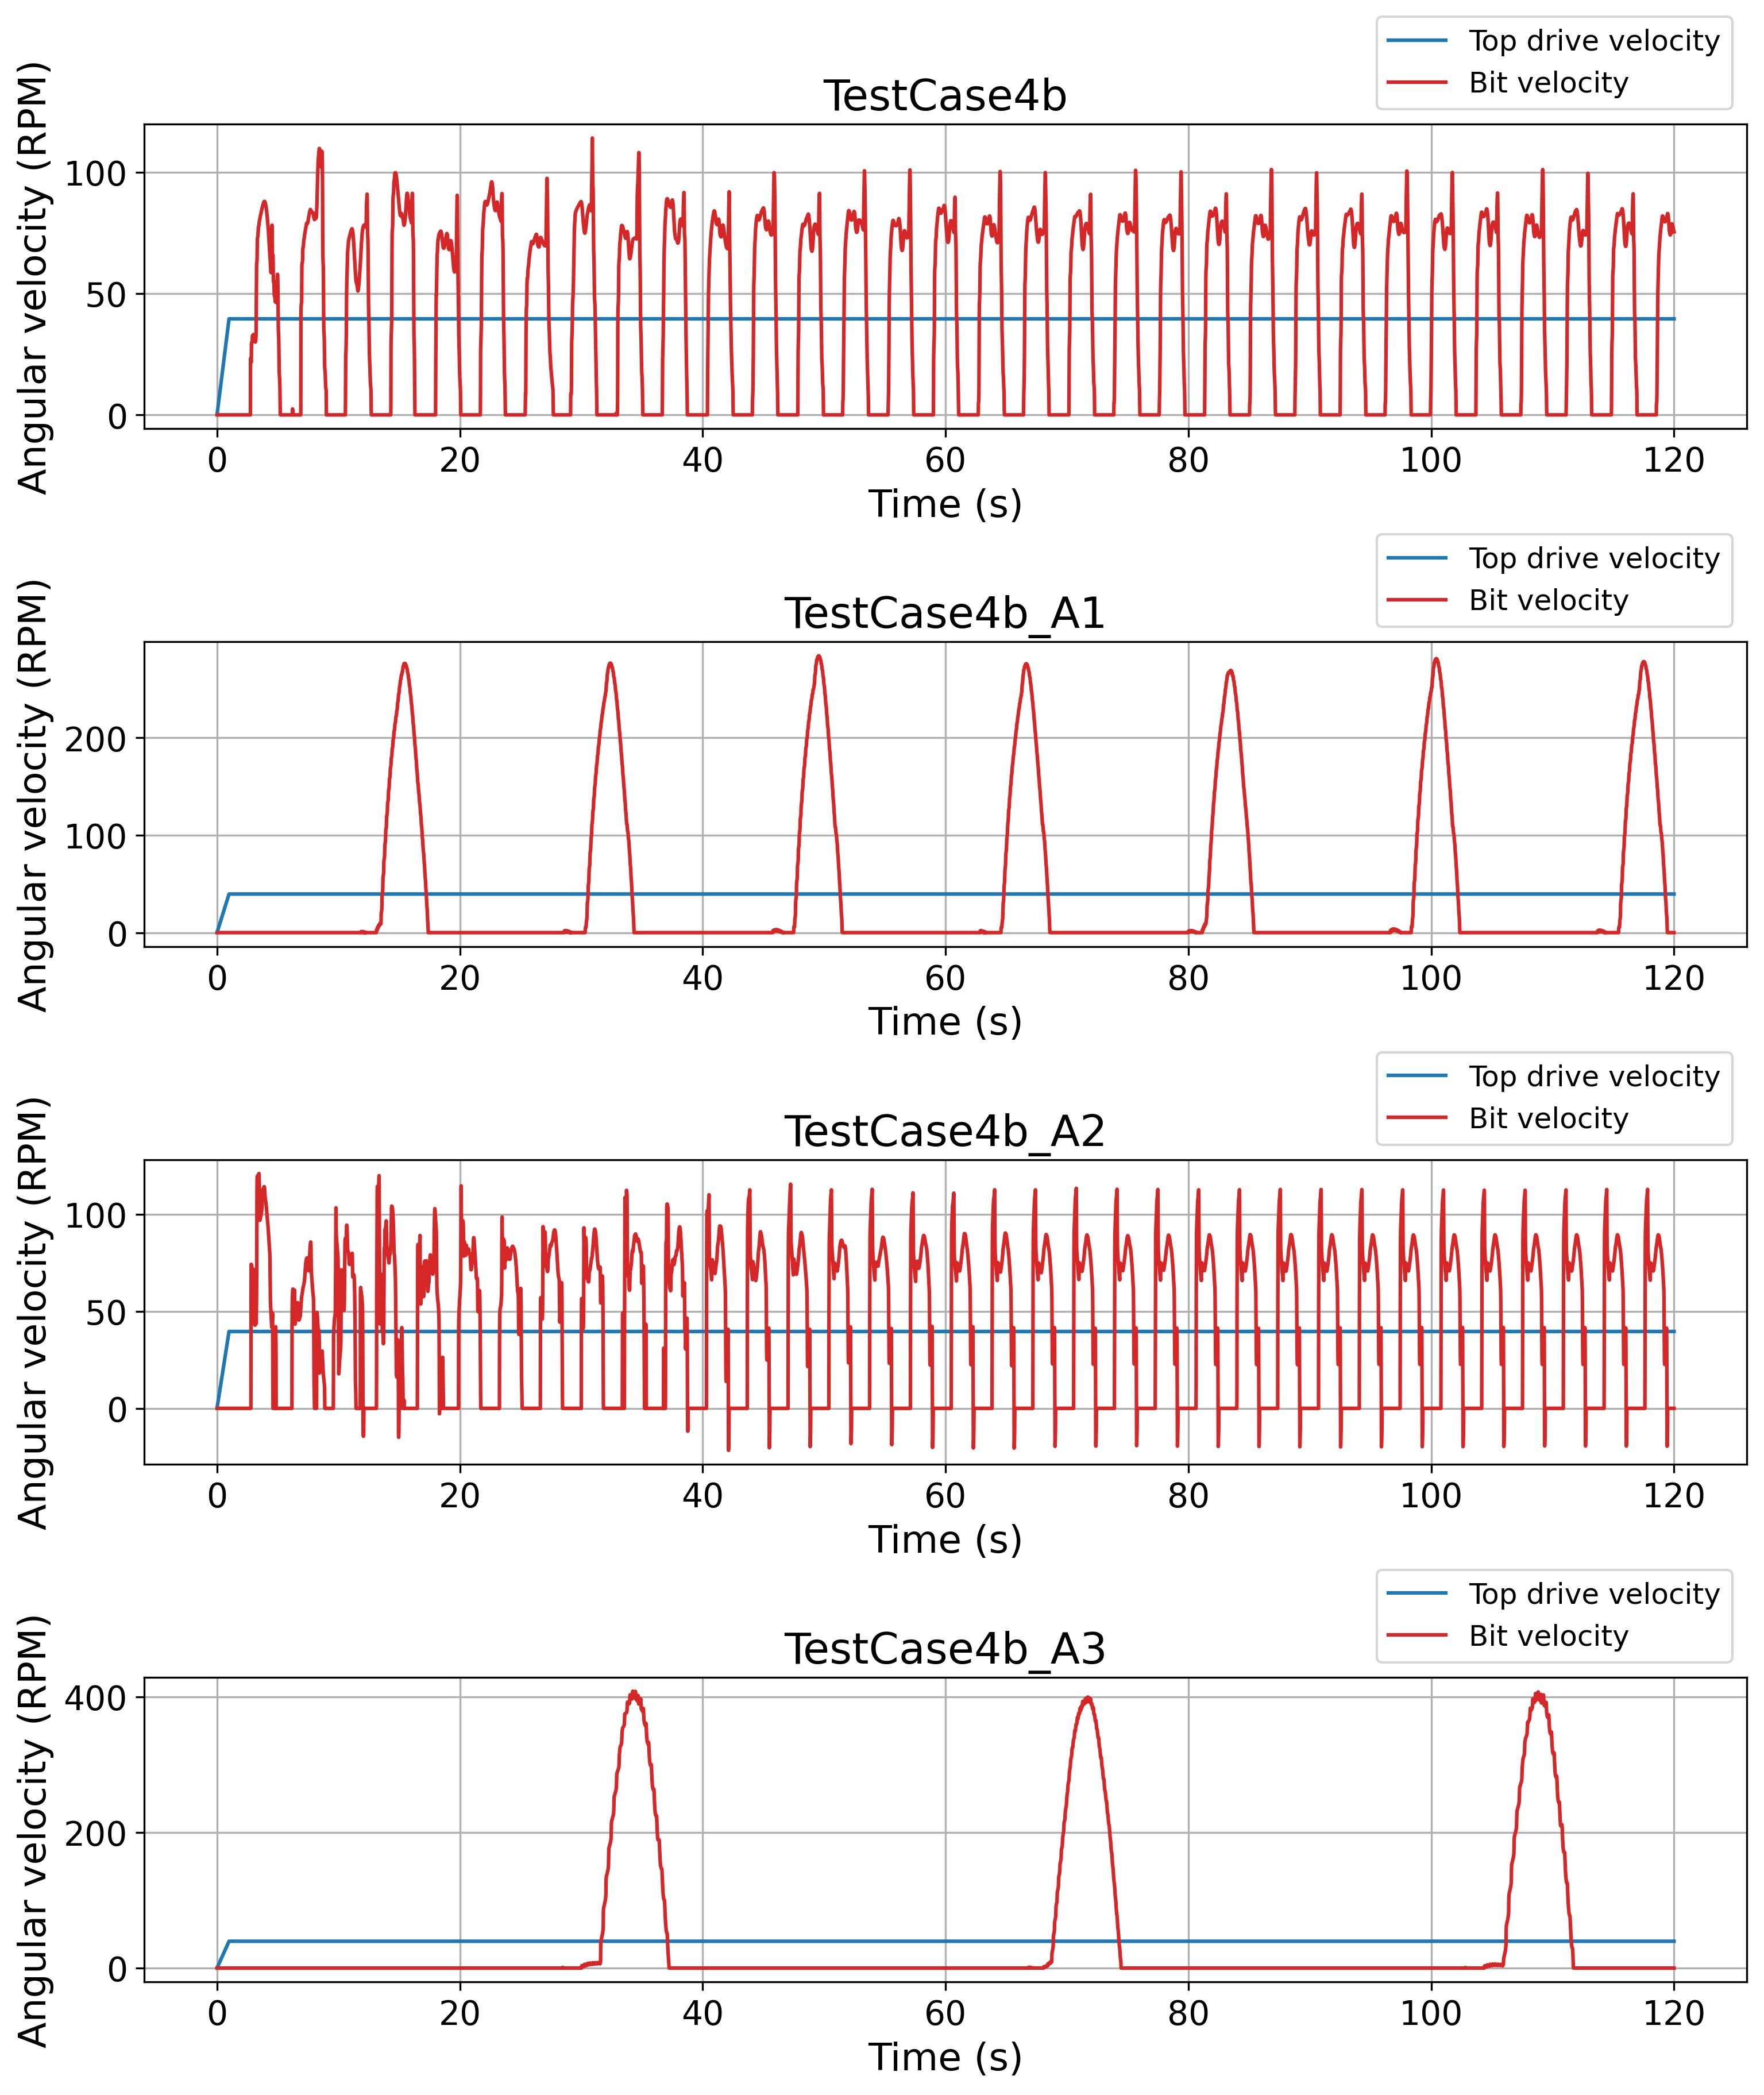
\includegraphics[width=\linewidth]{AS_size_effect_vel}
  \caption[Size effect of BHA components to angular velocity from A-S model]{Size effect of BHA components to angular velocity of bit from A-S model. The tests were conducted based on Test Case 4, where Test Case 4\_A1, Test Case 4\_A2 and Test Case 4\_A3 were simulated with doubled diameter, tripled length and both doubled diameter and tripled length of BHA components, respectively.}\label{figure_AS_BHA_size_effect_vel}
\end{figure}

\begin{figure}
  \centering
  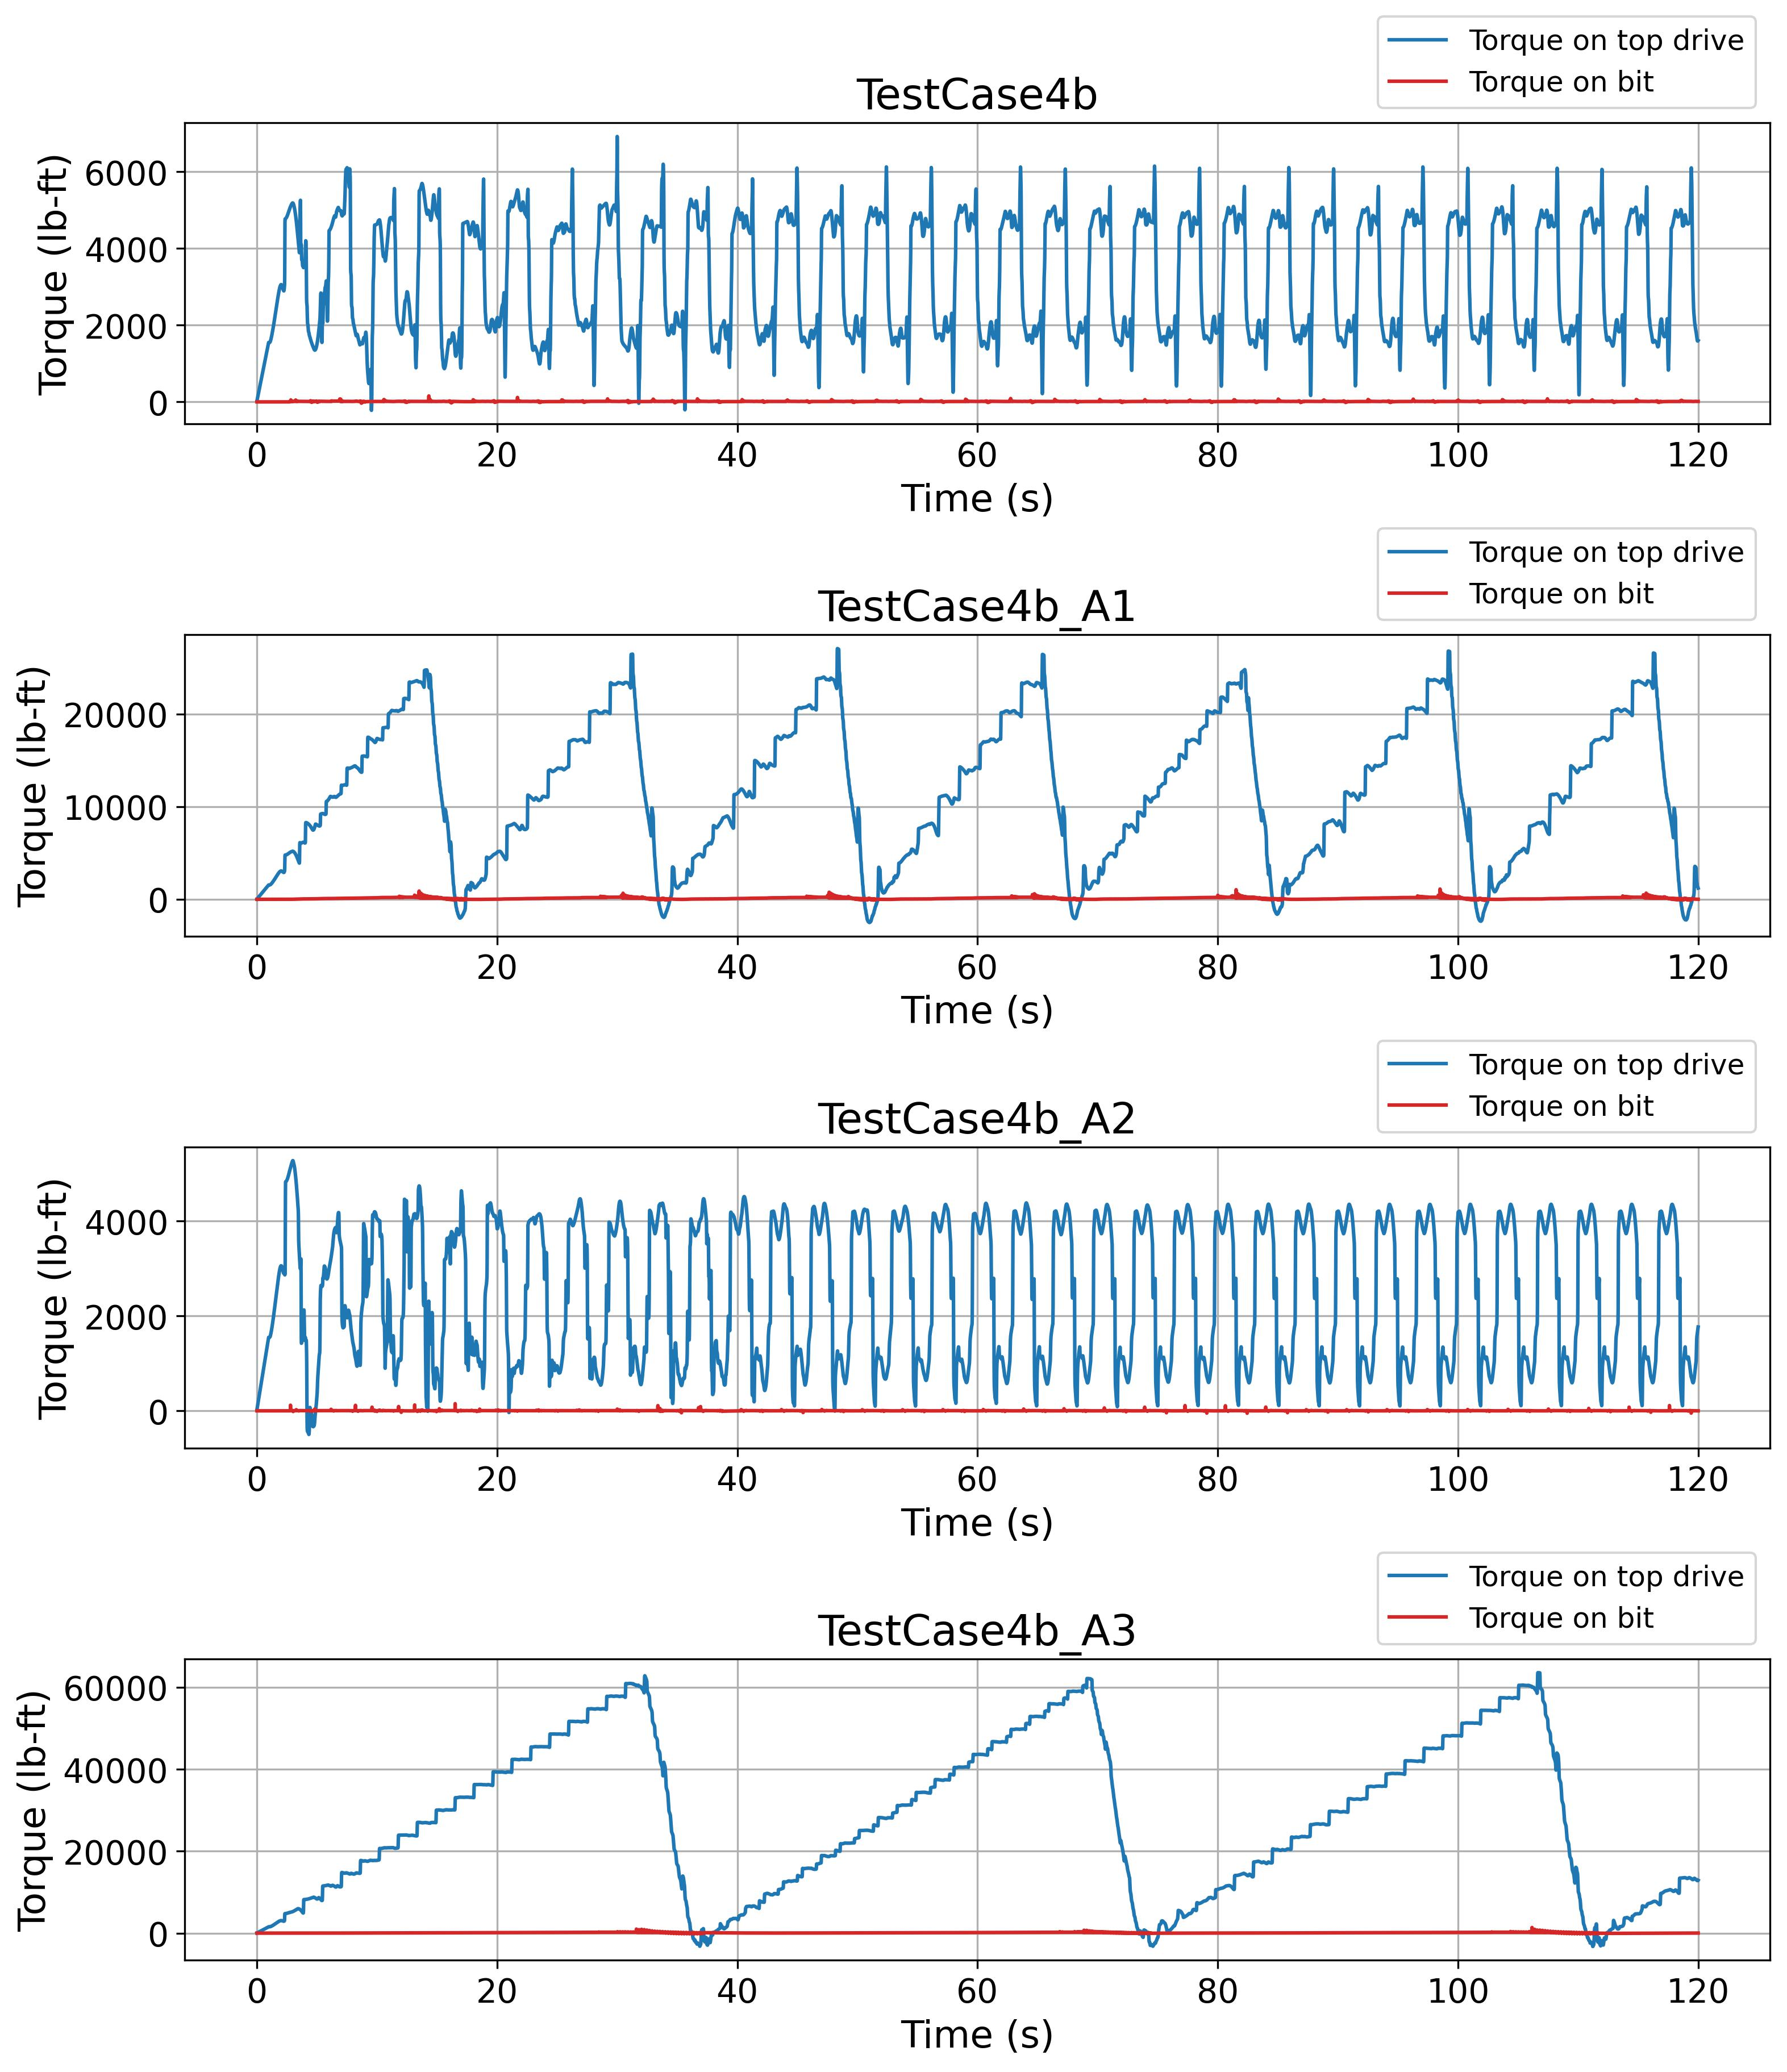
\includegraphics[width=\linewidth]{AS_size_effect_td}
  \caption[Size effect of BHA components to a torque from A-S model]{Size effect of BHA components to torque on top drive from A-S model. The tests were conducted based on Test Case 4, where Test Case 4\_A1, Test Case 4\_A2 and Test Case 4\_A3 were simulated with doubled diameter, tripled length and both doubled diameter and tripled length of BHA components, respectively.}\label{figure_AS_BHA_size_effect_td}
\end{figure}

\section{Effect of Shear Modulus} 